\documentclass[11pt]{report}

\usepackage[toc,page]{appendix}
\usepackage{amsmath}
\usepackage{stmaryrd}
\usepackage{syntax}
\usepackage{tikz}


\usetikzlibrary{shapes,arrows}
\tikzstyle{internalStage} = [rectangle, draw, fill=blue!20, 
    text width=5em, text centered, minimum height=4em]
\tikzstyle{conversion} = [draw, -latex']

\title{LJSP - A LISP to asm.js compiler}
\author{Jan S\"ondermann}
\date{1st January 1900}

\newcommand{\eqdef}{\stackrel{\text{def}}{=}}%
\newcommand{\cpstrans}[1]{\ensuremath{\mathcal{K}\llbracket #1 \rrbracket}}

\begin{document}

\maketitle

% originality
% abstract
% what it is?
% acknowledgements

\tableofcontents

\chapter{Introduction}
\section{Motivation for LJSP}
\section{Scope}

\chapter{Background \& Existing Work}
\section{Technologies involved}
% AST
\subsection{javascript engines/interpreters, new generation, history}
\subsection{asm.js}
\subsection{LLVM, LLVM IR}
\section{Similar Languages}

\chapter{Requirements}
\section{User Requirements}
\section{System Requirement}

\chapter{Specification}
\section{LJSP Grammar}
The grammar of LJSP in Extended Backus-Naur Form is given below.
\begin{grammar}
<program> ::= <defines> [ <expr> ] <defines>

<defines> ::= <define> <defines> | $\epsilon$

<define> ::= `(define (' <ident> <params> `)' <expr> `)'

<expr> ::= <double>
\alt <ident>
\alt `(if' <expr> <expr> <expr> `)'
\alt <lambda>
\alt `(let (' <letblocks> `)' <expr> `)'
\alt `(' <primOp> <args> `)'
\alt `(' <expr> <args> `)'

% add scientific form
<double> ::= \texttt{-?(\textbackslash d+(\textbackslash.\textbackslash d*)?|\textbackslash d*\textbackslash.\textbackslash d+)}

<ident> ::= \texttt{[a-zA-Z=*+/\textless\textgreater!?-][a-zA-Z0-9=*+/\textless\textgreater!?-_]*}

<lambda> ::= `(lambda (' <params> `)' <expr> `)'

<params> ::= <ident> | <ident> <params>

<letblocks> ::= <letblock> | <letblock> <letblocks>

<letblock> ::= `(' <ident> <expr> `)'

<primOp> ::= `+' | `-' | `*' | `/' | `neg'
\alt `<' | `>'
\alt `min' | `max'
\alt `sqrt'

% is an application to an empty argument list legal?
<args> ::= <expr> | <expr> <args>
\end{grammar}

The grammar for expressions used in intermediate stages is as follows:
\begin{grammar}
<expr> ::= <env>
\alt `(make-lambda' <lambda> <env> `)'
\alt `(nth' <int> <expr> `)'
\alt `(get-env' <expr> `)'
\alt `(get-proc' <expr> `)'
% should this be <expr> instead of <env>?
\alt `(hoisted-lambda' <ident> <env> `)'

<env> ::= `(make-env' <idents> `)'

<int> ::= \texttt{-?(0|[1-9][0-9]*)}

<idents> ::= <ident> <idents> | $\epsilon$
\end{grammar}

% subset of scheme
\section{Small/big-step semantics of LJSP}
\section{Backend Output}

\chapter{Design}
This chapter will describe @@@, this chapter: abstract, theoretical next chapter: concrete, details
\section{Overall architecture}
The compiler is made up of two major components: A hierarchy of classes that get instantiated to create the Abstract Syntax Tree (AST) @described in detail below@ and a number of compilation stages that perform various transformation on this AST. I will first describe the AST classes before going through all the individual stages of the compiler in detail.
% scheme is used for all internal code
\section{AST}
% class diagrams for all five sets of AST classes
The compiler includes five sets of class hierarchies that all have their own abstract superclass: One that reflects LJSP code, one for an intermediate representation used at a later stage and one for each compilation target: asm.js, C and LLVM IR.
\section{Detailed design of compilation stages}

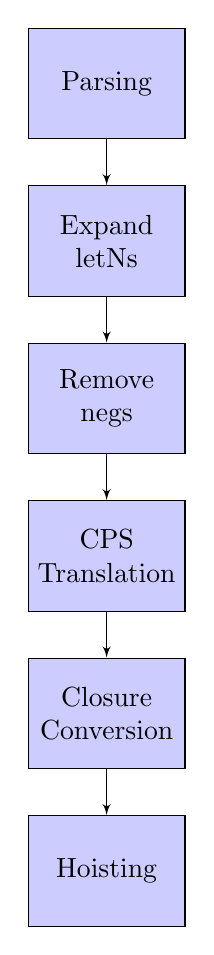
\begin{tikzpicture}[node distance = 2cm, auto]
    % Place nodes
    \node[internalStage](parsing){Parsing};
    \node[internalStage, below of=parsing](expandLetNs){Expand letNs};
    \node[internalStage, below of=expandLetNs](removeNegs){Remove negs};
    \node[internalStage, below of=removeNegs](cpsTrans){CPS Translation};
    \node[internalStage, below of=cpsTrans](clConv){Closure Conversion};
    \node[internalStage, below of=clConv](hoisting){Hoisting};

    
    \path[conversion] (parsing) -- (expandLetNs);
    \path[conversion] (expandLetNs) -- (removeNegs);
    \path[conversion] (removeNegs) -- (cpsTrans);
    \path[conversion] (cpsTrans) -- (clConv);
    \path[conversion] (clConv) -- (hoisting);

%    \node [block] (init) {initialize model};
%    \node [cloud, left of=init] (expert) {expert};
%    \node [cloud, right of=init] (system) {system};
%    \node [block, below of=init] (identify) {identify candidate models};
%    \node [block, below of=identify] (evaluate) {evaluate candidate models};
%    \node [block, left of=evaluate, node distance=3cm] (update) {update model};
%    \node [decision, below of=evaluate] (decide) {is best candidate better?};
%    \node [block, below of=decide, node distance=3cm] (stop) {stop};
%    % Draw edges
%    \path [line] (init) -- (identify);
%    \path [line] (identify) -- (evaluate);
%    \path [line] (evaluate) -- (decide);
%    \path [line] (decide) -| node [near start] {yes} (update);
%    \path [line] (update) |- (identify);
%    \path [line] (decide) -- node {no}(stop);
%    \path [line,dashed] (expert) -- (init);
%    \path [line,dashed] (system) -- (init);
%    \path [line,dashed] (system) |- (evaluate);
\end{tikzpicture}

% based on from system F...
\subsection{Parsing}
\subsection{CPS-Translation}

% y = var, i = int, f = fresh idn
\begin{figure}[ht]
\begin{alignat*}{2}
&\cpstrans{y} k &&\eqdef k(y) \\
&\cpstrans{i} k &&\eqdef k(i) \\
&\cpstrans{(\text{if}\ e_1\ e_2\ e_3)} k &&\eqdef \cpstrans{e_1} (\lambda x.(\text{if}\ x\ \cpstrans{e_2}k\ \cpstrans{e_3}k))) \\
&\cpstrans{(\text{lambda}\ (p_1, p_2, \dots, p_n)\ e)} k &&\eqdef k((\text{lambda}\ (cont, p_1, p_2, \dots, p_n)\ \cpstrans{e}cont)) \\
&\cpstrans{(\text{define}\ (name, p_1, p_2, \dots, p_n)\ e)} k &&\eqdef k((\text{define}\ (name, cont, p_1, p_2, \dots, p_n)\ \cpstrans{e}cont)) \\
&\cpstrans{(proc\ p_1, p_2, \dots, p_n)} k &&\eqdef \cpstrans{proc} \lambda x_{proc}.(\cpstrans{p_1} \lambda x_1.(\cpstrans{p_2} \lambda x_2. \dots \cpstrans{p_n} \lambda x_n.(x_{proc}\ x_1, x_2, \dots, x_n))) \\
&\cpstrans{(primitive\ p_1, p_2, \dots, p_n)} k &&\eqdef \cpstrans{p_1} \lambda x_1.(\cpstrans{p_2} \lambda x_2. \dots \cpstrans{p_n} \lambda x_n.(primitive\ x_1, x_2, \dots, x_n)) \\
&\cpstrans{(\text{let}\ ((idn\ e_1))\ e_2)} k &&\eqdef \cpstrans{e_1} \lambda x_1.(\text{let}\ idn = x_1\ \text{in}\ \cpstrans{e_2} \lambda x_2.(k(x_2)))\\
\end{alignat*}
\end{figure}


\subsection{Closure Conversion}
\subsection{Hoisting}
\subsection{Conversion to asm.js}
\subsection{Code emission}

\chapter{Implementation}
\section{Scala}
\section{Problems encountered \& resolved}
% variables that contain functions, ftables generated at compile time
\section{Experimentation \& Optimisation}
% array index vars of type int, others of type double
% (array index vars are all generated, user doesn't see them)

\chapter{Testing}
This chapter describes the methods that were used to test the different subsystems of the LJSP compiler. While testing is imperative for all software development projects, it is especially important in compiler development. The reason for this is that it is usually impossible to determine whether or not the result given by the compiler is correct simply by looking at the generated code. \\

During the development of LJSP, two means of testing were being used:
\begin{itemize}
\item A custom testing framework written in Python that covers all of the frontend stages and some of the backend stages.
\item A ray tracer written in JavaScript that was used to test generated asm.js code specifically.
\end{itemize}
The following two sections will describe both systems in detail.

\section{Testing using \texttt{run_tests.py}}
Early on in the development of LJSP, it became necessary to test the output of every front end stage 
\section{Testing using the ray tracer}
% because asm.js evaluates to the same result regardless of
% whether or not it's compiled according to asm.js specification,
% it's possible to add invalid statements and still test the module

% ray tracer to test performance

\chapter{Evaluation}
% ast transformations would be nicer if the compiler generated the subtrees
% from short code snippets instead of creating the objects manually
\section{Evaluation against requirements}
\section{Strengths \& Weaknesses}

\chapter{Professional Issues}
% http://www.bcs.org/category/6030

\chapter{Conclusions}
\section{Future Work}
\subsection{Optimisations}
\subsection{Types}

\chapter{Bibliography}

\begin{appendices}

\chapter{Userguide}
\section{CLI switches}
% how to run tests

\chapter{Class diagrams}

\chapter{Programs Listings}

\end{appendices}

\end{document}
